\documentclass{beamer}
\XeTeXlinebreaklocale "zh"
\XeTeXlinebreakskip = 0pt plus 1pt

\usetheme{CambridgeUS}
\usepackage[most]{tcolorbox} 
\usepackage{fontspec}
\usepackage{tikz}
\usepackage{amsmath, amssymb}
\setmainfont{Noto Serif CJK TC}
\setsansfont{Noto Sans CJK TC}
\setbeamertemplate{background}{
    \tikz[overlay, remember picture]\node [opacity=0.2] at(current page.east)[below=2cm, left = 0.2cm]{
\includegraphics[width=4cm]{logo.png}};
}

\AtBeginSection[]
{
 \begin{frame}<beamer>
 \frametitle{Outline}
 \tableofcontents[currentsection]
 \end{frame}
}
\AtEndDocument{\begin{frame}
\centering \Huge
                  Q \& A
               \end{frame}
                }
\title{Research on zk-SNARK}

\begin{document}
\begin{frame}
\titlepage
\end{frame}

\frame{\frametitle{Outline}
\tableofcontents%[pausesections]
}
\section{zkSNARK背景知识}
\begin{frame}\frametitle{二元算数电路(QAP)证明}
\begin{itemize}
\item Every program can be extracted as a quasi arithmetic circuit.
\item To prove an array of signals (inputs/outputs) makes a program proved.
\end{itemize}
\begin{tcolorbox}[enhanced,colframe=white,colback=white, fuzzy halo = 1.3mm with gray]
\centering
\usetikzlibrary{trees}
	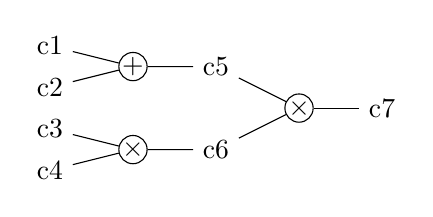
\begin{tikzpicture}[grow=left,
	level 2/.style={sibling distance=3em},
	level 4/.style={sibling distance=1.5em}, level distance=3em]
		\node {c7}
		child { node [draw, circle, inner sep=0mm]{$\times$}
		child {node {c5}
		child {node [draw, circle, inner sep=0mm]{$+$}
		child {node {c1}}
		child {node {c2}}
		}}
		child {node {c6}
		child {node [draw, circle, inner sep=0mm]{$\times$}
		child {node {c3}}
		child {node {c4}}
		}}
		};
	\end{tikzpicture}
	\begin{itemize}
	\item A set of signals (e.g., c1 and c7\footnote{称为statement}) are public
	\item The goal of snark is to prove other ``secret'' signals\footnote{称为witness} can express the circuit. 
	\end{itemize}
\end{tcolorbox}
\end{frame}

\frame{
\frametitle{High-level Protocol}
\begin{enumerate}
\item 每个client上传自己的梯度给T(密文)
\item T得到这一轮的平均梯度 (如任务的隐私不重要,可明文)
\item 每个client证明自己的余弦距离是近的
\item 有证明能力的client具有继续下一轮训练的能力
\end{enumerate}
}

\section{Prelimiries}
\frame{\frametitle{Bilinear Pairing}
A mapping $e$ works on three order-$q$ groups ($\mathbb{G}_1, \mathbb{G}_2, \mathbb{G}_T$) as $$e: \mathbb{G}_1\times \mathbb{G}_2 \rightarrow \mathbb{G}_T$$

\begin{tcolorbox}[enhanced,colframe=white,colback=white, fuzzy halo = 1.3mm with gray]
\begin{enumerate}
\item \textcolor{red}{Bilinearity}. $\forall a, b \in \mathbb{Z}_p^2$, $u, v\in \mathbb{G}_1\times \mathbb{G}_2$: $e(u^a, v^b) = e(u,v)^{ab}$
\item \textcolor{red}{Non-degracy}. $u$ and $v$ are generators of $\mathbb{G}_1$ and $\mathbb{G}_2$: $e(u,v)$ generates $\mathbb{G}_T$.\footnote{$e(u,v)$的所有幂次取遍群里的所有元素}
\item \textcolor{red}{Efficiency}. $e$ is a polynomial-time algorithm for all $u,v$.
\end{enumerate}
\end{tcolorbox}
}

\frame{\frametitle{Lagrange Interpolation}
Any degree-$t-1$ polynomial $$P(x) = \sum_{i=0}^{t-1} a_i x^i$$
can be reconstructed from $t$ distinct points in the curve \footnote{Instance: a degree-2 curve is determined by 3 points}. 

\begin{tcolorbox}[enhanced,colframe=white,colback=white, fuzzy halo = 1.3mm with gray]
With $t$ points $(x_i, y_i = P(x_i))$
$$P(x) = \sum_{1\leq i\leq t} l_i x_i$$
$$ l_i = \prod_{1\leq j\leq t}^{j\neq i} \frac{x - x_j}{x_i - x_j} $$
\end{tcolorbox}
}

\end{document}
